\documentclass{report}
\usepackage[utf8]{inputenc}
\usepackage{natbib}
\usepackage{graphicx}
\usepackage{float}
\usepackage{url}
\usepackage{commath}
\usepackage{gensymb}
\usepackage[affil-it]{authblk}
\usepackage[colorlinks,allcolors=blue]{hyperref}
\usepackage{algorithm}
\usepackage{algpseudocode}

\citestyle{acmauthoryear}
\setcitestyle{square} 

\title{Realtime Environment Lighting Simulation for Augmented Reality Applications}
\author{Marco Antonio Salcedo Sanson%
}
\affil{Utrecht University, Faculty of Science, Game and Media Technology Master's Program}

\author{Supervised by Amir Vaxman%
}
\affil{Department of Information and Computing Sciences, Utrecht University}

\date{Dated: \today}

% Definition of \maketitle
\makeatletter         
\def\@maketitle{
\noindent
\begin{center}
{\huge \bfseries \sffamily \@title }\\[4ex] 
{\Large  \@author}\\[4ex] 
\@date\\[8ex]
\end{center}}
\makeatother


\begin{document}
\begin{figure}[t]
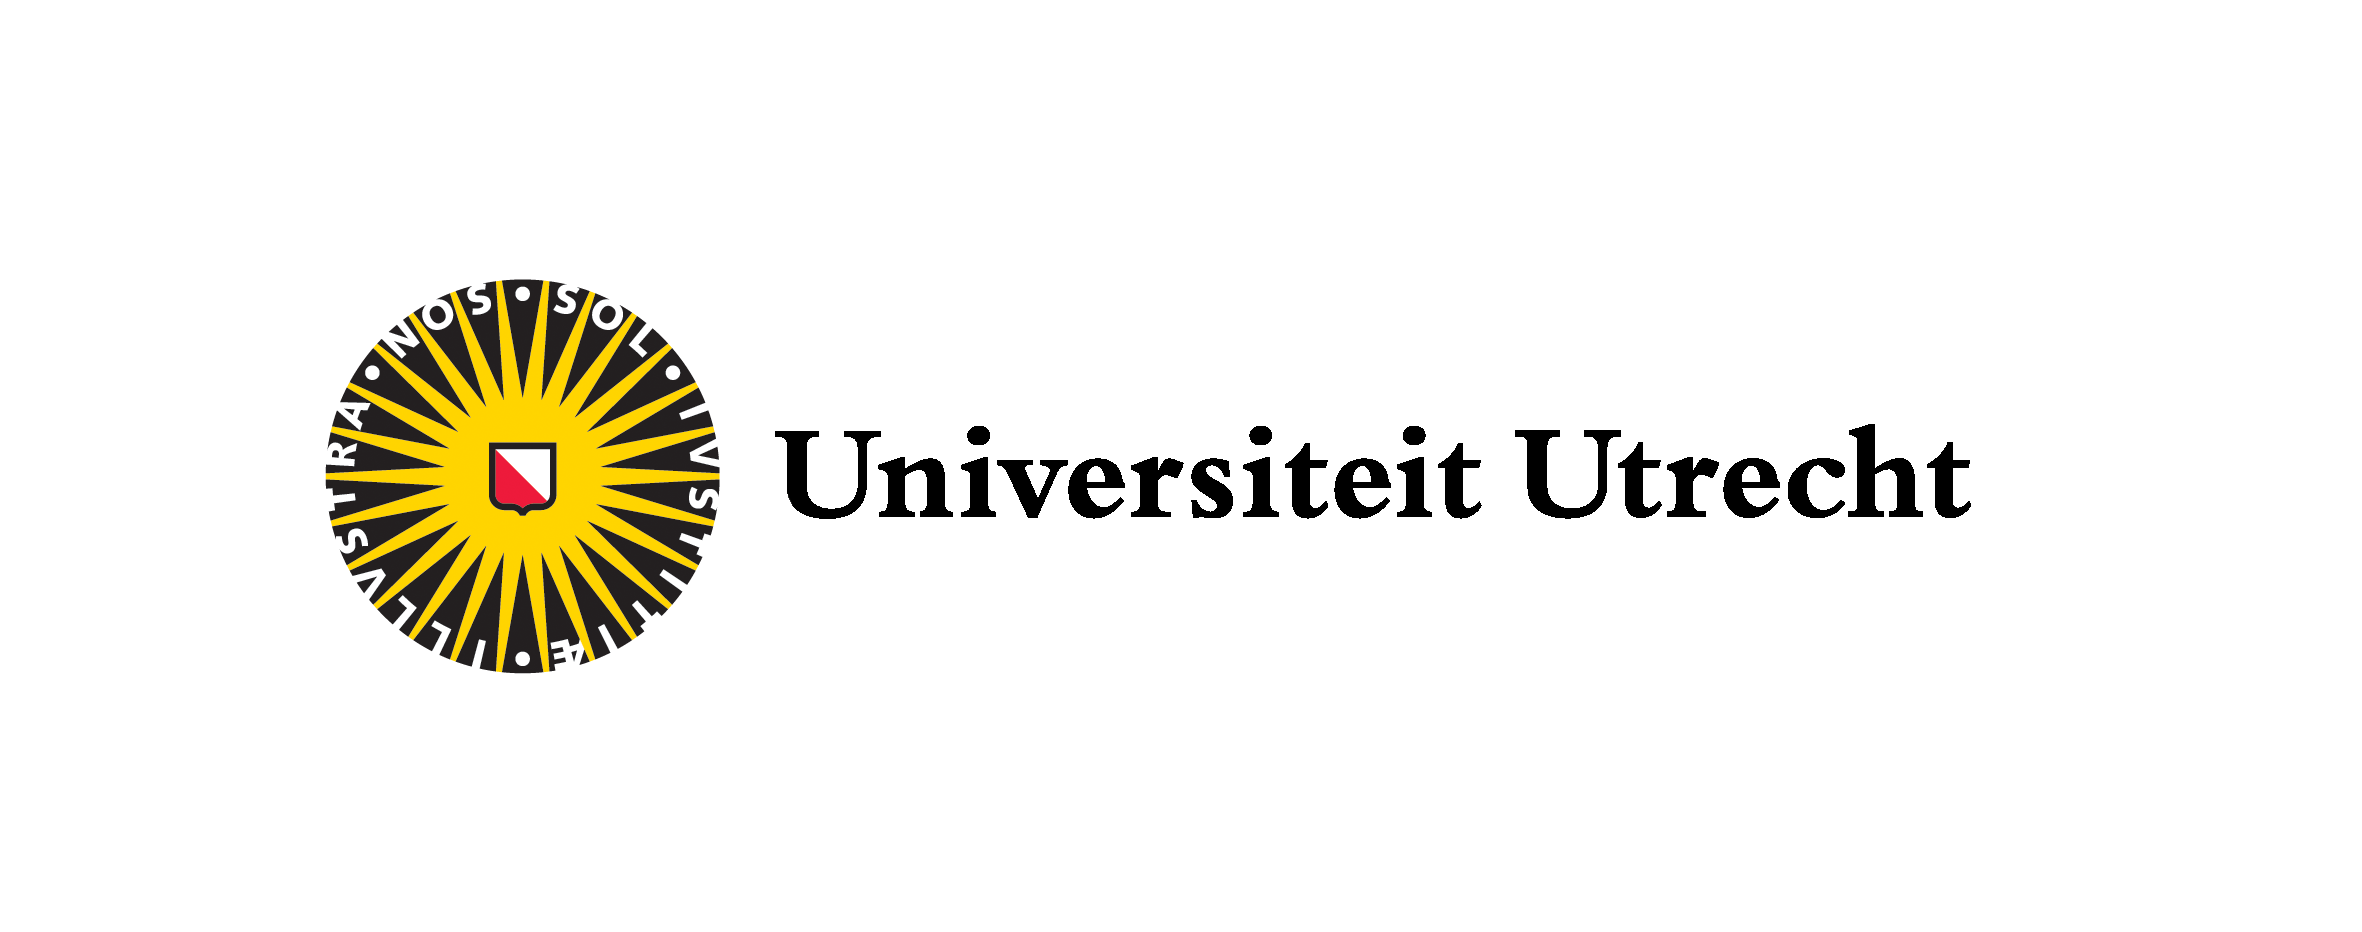
\includegraphics[scale = 0.5]{Figures/uu-logo.png}
\end{figure}

\maketitle
\clearpage

\tableofcontents{}
\clearpage

\chapter{Introduction} \label{introduction}
%!TEX root = ../main.tex

The rendering of virtual objects on current AR applications has a number of shortcomings in the state of the art. It is quite easy to tell that it’s a superimposed virtual object. There are many factors that come into play and give away the lack of feasibility of an AR object, such as marker jiggle, inaccurate depth cues, lack of occlusion from real life objects and incompatible lighting.
The method proposed in this work addresses the latter problem, the incompatible light conditions of the virtual and real world. The method is based on the idea that a 360 photograph of the environment can give us a lot of information about the lighting conditions and that such 360 photographs are now simple to create on an average mobile device. From this 360 photograph it can be determined if the environment is outdoors by day or any other case of illumination. If the environment is indoors the light sources of the room will be approximated using the photo, if outdoors the sun will be assumed as the main source of light, and its position would be calculated using the clock, calendar and compass of the mobile device running the application. \newline
Whatever the case, the method's output is a set of lights whose properties are a position relative to the camera, a rotation, color, type of light (spotlight or area light) and an intensity.
It's important to stress the fact that the method is proposed for mobile devices. There have been previous works, detailed in the next chapter, that deal with the same problem but on computers. Mobile devices present advantages over computers for this task, but also the downside of generally lower processing power compared to computers. This decision comes from the ease of producing the 360 photographs locally, from the judgement that AR is better suited for mobile devices than computers (for mobility and ease of use reasons) and also to be able to exploit the devices geolocation hardware. Of course this doesn't mean that the method will only be applicable to mobile, there are also ways to adapt it to work on computers too.\newline
The research question from which this method was originally envisioned is: "Can the accuracy of lighting in AR applications be improved using a mobile device to it's full potential?". What this means is that thanks to the many ways a smartphone or tablet can interact with the user and the environment we can know a lot about the surroundings. And this information could potentially be very useful to save computation time, which will make up for the lower computational capabilities and make for a more fair comparison to other methods.\newline
The contributions of this method are:
\begin{itemize}
    \item An image-based method with which the lighting conditions of the full visible environment can be modeled
    \item The use of the mobile device's geolocation hardware to enhance the light simulation with the knowledge of the current weather conditions and the position of the sun
\end{itemize}


\chapter{Related Work} \label{related}
%!TEX root = ../main.tex

Agusanto et al. proposed a similar method \cite{agusanto2003}. The main differences in the method they propose have to do mostly with the technologies used. Being already an old paper, their method was conceived for Augmented Reality on a computer, rather than on a smartphone. The choice of a smartphone comes with the downside of lower processing power, but with the great advantage of the different sensors available on the device. The method in the Agusanto paper infers the lighting conditions using hand-crafted HDR photographs of the real scene using highly reflective metal spheres in contrast with my proposition of using the 360 degree photograph on the device itself, which is a lot more accessible to an average consumer.\newline
Pessoa\cite{pessoa2011} expanded on Agusanto's work and created the Real-Time Photorealistic Rendering of Synthetic Objects into Real Scenes (RPR-SORS) toolkit as an extension of the ARToolkit Augmented reality SDK. Although they use more modern techniques, such as cubemaps instead of HDR photographs, their approach still has the same differences than the Agusanto method.\newline
There have been several methods to insert virtual objects into static photographs automatically with highly realistic results. One such example is the method by Karsh \cite{karsh2014} These kind of methods are not suitable for real- time applications, and they use a single view image to infer the lighting conditions. The method proposed here is more robust in the sense that it uses a 360 view of the environment to eliminate assumptions of what there is out of frame.\newline
Xing\cite{xing2013} also devised a method to compose virtual objects into static photographs, focusing on outdoors scenes. The method is quite sophisticated, but a lot of the information fed to the light calculation functions involve manual input by the user. The proposed method is intended to work both for indoors and outdoors scenes, the main difference with the way outdoors scenes will be managed is that the method works automatically, without user intervention. This is accomplished by the usage of the mobile device's dedicated geolocation hardware. By using it, there is no need to assume anything or ask for any user input, the device will be able to tell a good approximation of the sun position using only the sensor's information.

\chapter{Theoretical Framework} \label{theory}
%!TEX root = ../main.tex

In this section a few technical concepts will be explored in order to make the proposed method and what it aims to accomplish more clear.

\textbf{Augmented Reality}\newline
As of yet, the definition of Augmented Reality that is most widely accepted is the one presented by Azuma\cite{azuma1997}. In this survey Augmented Reality (or AR for short) is defined as a software system that features a blend of real and virtual objects, the user can interact with it in real time and presents a 2D representation of a 3D world for both the real and virtual sides. A feature film that integrates real and virtual characters or objects is therefore strictly speaking not AR for example, because it's static content, the consumer cannot interact with it at all, let alone in real time.
In order to combine real and virtual objects both worlds must be aligned, in the sense that they must share a common origin for both position and rotation. If the virtual objects present in the real scene are not aligned the feasibility of the whole composition is compromised. The tracking of real world features as a guideline for alignment in the virtual world is one of the challenges in the field of AR. There are many techniques that have been used, such as sensor-based tracking, that uses dedicated hardware to feed the software application the position and rotation information it needs; vision-based tracking, in which the position and orientation origin of the virtual world are determined by images recognized by a computer vision algorithm. These images are named fiducial markers and can be an artificial black and white image, a "natural" images (points, lines, shapes and/or textures) or even 3D objects. Other approaches involving both sensors and vision algorithms have also been used, if the reader is interested in learning more about tracking, Zhou's survey\cite{zhou2008} on tracking is a good resource.
This method does not aim in any way to improve tracking for AR, current state-of-the-art methods will be used for that, but it's important to explain the concept a bit in order to settle the scope and expectations of the end result.

\textbf{Sensors}\newline
Most smartphones and tablets in the market nowadays have built-in sensors to measure many things that are helpful for application developers, such as motion, orientation and other environmental conditions. The ones that are relevant for this method are the following:\newline
\textbf{Accelerometer}: This device measures proper acceleration relative to gravity. Its application in mobile development is to measure motion changes and to measure the device orientation relative to Earth's surface. It usually consists of 3 orthogonal axes. The output is given in m/s\textsuperscript{2} \newline
\textbf{Gyroscope}: A sensor that is capable of measuring the rate of rotation around a particular axis. It serves the same purpose as the accelerometer, but mobile devices usually have both for more robust measurements. The output is given in rad/s. In the method these will be used to acquire the 360 panoramic photograph, making sure that the device is within the same pitch while capturing all the images that will be stitched together to make the panorama. \newline
\textbf{Photometer}: There is a wide variability in terms of capacity of photometers across different devices, but the only measurement that is guaranteed is the ambient illuminance expressed in lx.  In the method it will be useful for detection of a noticeable change in ambient lighting, leading to a re-capture of the panorama. What exactly constitutes a noticeable change in ambient lighting will be determined through parameter tuning. \newline 
\textbf{Magnetometer}: In terms of mobile devices it serves the purpose of a compass, it measures the device's orientation with respect to the Earth's magnetic poles. In mobile development it is useful to get the heading of the device expressed in degrees.\newline
\textbf{GPS}: Measures the raw position of the device in three-dimensional Cartesian coordinates with origin on the center of the Earth. It can be used to determined where on planet Earth the device is located (Country, city, neighborhood, etc). It needs to have line of sight with no electromagnetic interference with at least 4 out of the 24 satellites in orbit that are used for GPS.

\chapter{Methodology} \label{method}
%!TEX root = ../main.tex
%TODO: Redo the flowchart with updated and more specific steps

This chapter covers the steps needed to produce the wanted results. The input needed is a fiducial marker $M$ to provide the object position in the real world; and a 3D mesh $O$ which will be rendered in Augmented Reality. The output is a set of light sources $L_i$, each one having a position, orientation, intensity, color, type and size. In order to complete the luminance ($L()$) analysis a 360 panoramic image is required, but it will be generated in a previous step with a separate application as explained in the Theoretical Framework chapter. The entirety of the process is layed out in the flowchart in Figure 1, and each step is described in more detail afterwards.

\begin{figure}[H]
  \centering
  \setlength{\unitlength}{\textwidth} 
    \begin{picture}(1,0.5)
       \put(-0.1,0){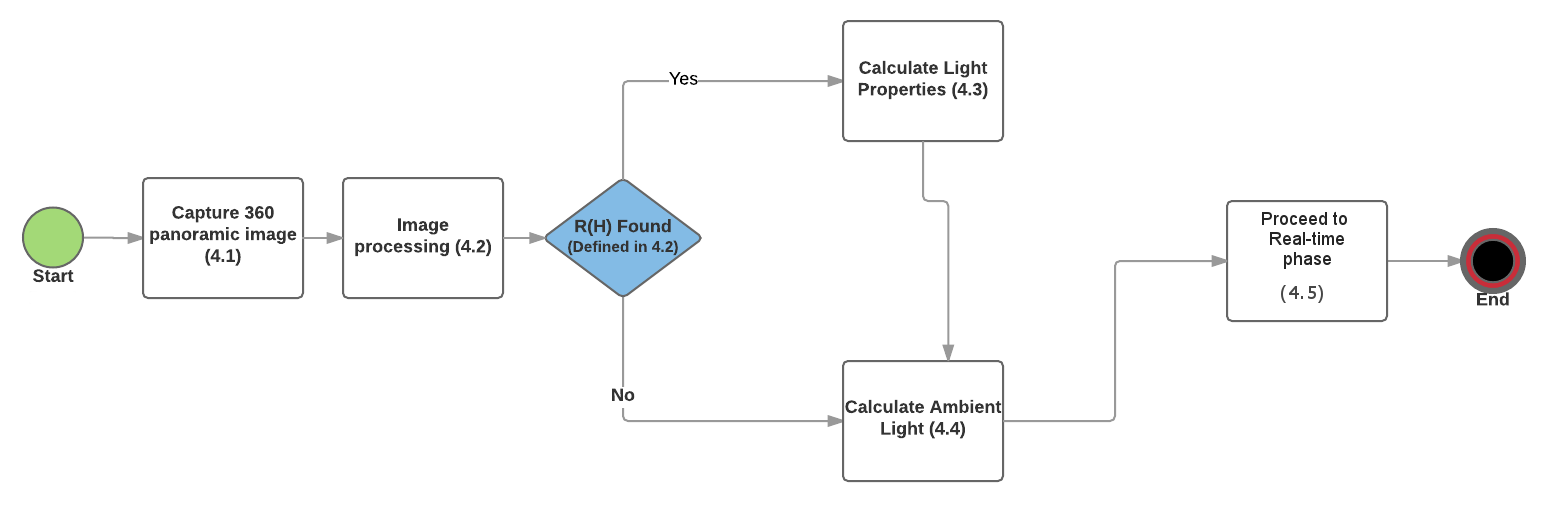
\includegraphics[width=1.3\unitlength]{Figures/Flowchart.png}}
       
    \end{picture}
    \caption{The method in a nutshell}
\end{figure}

\section{Capture 360 panoramic image}
In this work panoramic images are used as a tool, therefore it's not within the scope of the method to define a new way of capturing 360 images. The suggested application to procure a spherical panoramic image within the device itself is Google Street View.
The origin of the virtual world for placing and orienting $O$ within it is asked to the user by rotating the virtual reflective sphere so that the texture offset matches the device orientation within the real world. This will also simplify calculations of light orientations later on.

\section{Image processing}
Once the panoramic image is loaded and oriented the first step in order to be able to analyze the luminance is to get rid of the chromatic information. This is achieved with the following equation:

\begin{equation}
    L(R_{ij},G_{ij},B_{ij}) = 0,2126 \times R_{ij} + 0,7152 \times G_{ij} + 0,0722 \times B_{ij}; \quad \forall \  P_{ij}
\end{equation}

Where $L$ is the luminance obtained at D65 white point and $P$ is the pixel in the $i,j$ position of the image \newline
The contrast ratio has to be adjusted, so that the regions with high luminance are more clearly differentiable. 

\begin{equation}
     g(i,j) = \alpha \times f(i,j) + \beta
\end{equation}

Where $g(i,j)$ is the adjusted image, $f(i,j)$ is the original grayscale image and $\alpha$ and $\beta$ are the brightness and contrast constants, determined by parameter tuning. The parameter tuning will be carried out in a trial and error way, propose initial extreme values and run the program, changing the values in order to achieve the best result. The values that worked in the implementation were $\alpha = 220$ and $\beta = 255$.
In order to prevent outlier pixels and noise from causing false positives, let $g(i,j)$ be normalized like so:

\begin{equation}
    L(P_{ij}) = \frac{ 2 \times P_{ij} }{min(L) + max(L)}
\end{equation}

Where $min(L)$ and $max(L)$ are the overall minimum and maximum luminance values in the image. 
\newline
The result of these steps is a black and white image with the rough shape of the light source. If the image ends up completely black it means there are no important visible light sources and ambient illumination alone would give a good enough result on the rendered model. A region of high luminance is defined as follows:

\begin{equation}
    R(H) = \{p_{00}, p_{01}, ... , p_{mn}\}
\end{equation}
 Where $p_{ij}$ is the pixel in the i,j position of the image. Such that 
\[
    L(p_{ij}) > 0.9 \times max(L(p_{ij})) 
\]

The region must also be continuous, so the pixels must be adjacent.\newline
If there are regions of high luminance in the image, they would be discovered with a fair amount of noise and artifacts, caused by clear objects, reflections of light sources on highly reflective surfaces, or even light sources that are so far away in the distance that don't really contribute an important amount of light to the area of interest. Therefore it's necessary to also add a relative size constraint to the definition. What constitutes an acceptable region size to deem the light source is not an easy question to answer. The best approach to face this problem is to define it as a percentage of the width and height of the overall image and tune the parameter in search for the best solution. The size constraint would therefore be:

\begin{equation}
    width(R(H)) \times height(R(H)) \geq k \times W \times H
\end{equation}

Where $k$ is the parameter to be tuned, in the implementation the value that yielded the best results was $k = 0.004$; $W$ and $H$ are the total image width and height.\newline

These constraints also help keep the amount of lights to be processed within an acceptable range for a real-time application, even if the real environment has many light sources a simplification of them is necessary when modelling them to keep the application feasible. In the implementation the maximum amount of lights was capped to 8 because the overall performance of the application started to suffer with more lights. However, in order to identify the most relevant light sources it's necessary to calculate their parameters first.\newline
Once a set of light sources have been identified their properties need to be calculated.

\section{Calculate light properties}
The properties needed to calculate for each light are orientation, intensity and color. In the real world it is not trivial to calculate the position from just a single point of view as input, so even though the simulation would be a lot more robust if the actual position with respect to the camera was simulated there is just not enough information to calculate it in this method and all the lights are assumed to be at unit distance from the camera. With this in mind, all the other properties can be calculated.

\begin{enumerate}
\item Position:The x, y and z components will be those of the unit orientation vector, to ensure that the light is in the correct direction at unit distance.

\item  Orientation: The pixel coordinates (x,y) of the centroid of each light within the luminance panorama are saved. The image is projected on a sphere. The camera casts rays onto the sphere from 4 different points of view, 0\degree , 90\degree, 180\degree  and 270\degree. If the ray hits a white pixel and the pixel coordinates of the hit are approximately those of the centroid the light direction is calculated as follows:
\begin{equation}
    O(L_p) = -2 \times (N_h \cdot C_r) N_h + C_r
\end{equation}
Where $O(L_p)$ is the orientation of the pth light source, $N_h$ is the sphere normal on the hit point, $C_r$ and is the camera ray direction.
\item Color: Storing both versions of the panorama, one in full color and another one after processing will allow us to have both the color and the luminance information. Once a light source is detected, the equivalent area in the color image can be averaged to determine the color of the light source.
\item Intensity: There are two factors that influence the intensity of a light as perceived by a camera, the light size and the color temperature. The light's color temperature in Kelvin can be calculated as follows:
\begin{equation}
    T(C_p) = -949.86315 + 6253.80338 ^ {\frac{-n}{0.92159} } + 28.70599 ^{\frac{-n}{0.20039} } + 0.00004 ^ {\frac{-n}{0.07125} }
\end{equation}
\begin{equation}
n = {\frac{0.23881\times R + 0.25449\times G - 0.58291\times B}{0.11109\times R - 0.85406\times G + 0.52289\times B} }
\end{equation}

Where $R, G, B$ are the red, green and blue components of the light color.\newline 
The size analogy is given by the integral of the region of high luminance with respect to the full image. The light intensity is finally expressed by:
\begin{equation}
I(L_p) = T(C_p) \times \int_R L(i) \,dx
\end{equation}
Where $L(i)$ is the output image of the luminance analysis and $R$ is the pth region of high luminance.\newline 

\end{enumerate}

\section{Calculate ambient light}
Environment mapping is an image-based technique to approximate the appearance of the overall light conditions of an environment. This is accomplished by means of a precomputed texture image mapped as a far-away environment surrounding. Said surrounding is usually a geometric surface, when Blinn first introduced the method\cite{Blinn76} a sphere was used. Nowadays there are other alternatives, such as cube, paraboloid, pyramid or cylinder maps. The principle for each surface is the same, but the way to map a planar image onto the surface varies per surface.\newline
Since a panoramic image of the environment is already available using it to implement environment mapping would be an adequate use of resources. In order to generate an environment map it is necessary that the panorama is made into a High Dynamic Range image. This is because the Low Dynamic Range image captured directly from the device camera fails to capture the information necessary to simulate correct color balance, shadows, and highlights of the lighting environment; ultimately producing both inaccurate and less visually pleasing results. This has been illustrated by Paul Debevec.\cite{DebevecRSO}\newline 
A relatively easy and effective way to make an image into an HDR version is a technique called Tone Mapping, in which versions with different exposure values of the same image are blended together to include the full range of highlights and shadows of the overexposed and underexposed versions in a single image. Since asking the user to capture the environment more than once would have a bad impact on user friendliness, and also it's highly unlikely that the produced image would have the exact same framing every time, the different exposure values for the Tone Mapping will be produced altering the brightness and contrast values of the base image using equation 2 once again. After that the HDR image is produced using Debevec's weighting algorithm\cite{Debevec}.\newline
It's important to disclaim that the Tone Mapping process will not yield an actual HDR image. In the first place, it will be a standard 24 bit image in the $0...255$ range, with highlight and shadow valued clipped. The upside to still going through this process nonetheless is that the environment will be described in a richer way, capturing the bright areas and the shadows better than the standard exposure image.\newline
After the HDR version of the panorama is created it can be used to have an actual ground truth about the environment light color and intensity at any given point in the virtual space. This will be detailed in the Real-time Phase step subsection.

\section{Real-time Phase}
The original sphere panoramic photograph is widely used in the real time phase. It is used to create a cubemap of the real environment to be used as ambient lighting, to calculate the ambient contribution of the diffuse shaders and to fake reflections for the specular shaders.
\begin{enumerate}

\item Cubemap: The image coordinates are first converted to polar and divided into four regions by latitude $-\Pi/4 < \theta < \Pi/4 , \Pi/4 < \theta < 3\Pi/4, 3\Pi/4 < \theta < 5\Pi/4, 5\Pi/4 < \theta < 7\Pi/4$. These represent either one of the four faces of the cube, top or bottom. The projected coordinate is given by:
\begin{equation}
P = (1, tan(\phi), \frac{cot(\theta)}{cos(\phi)})
\end{equation}
 The projected point is always on the top if $ \frac{cot(\theta)} { (1/\sqrt{2}) }> 1$ or $tan(\theta)< \frac{1}{\sqrt{2}}$ \newline
 
 The projected points for each face of the cube are composed into an image and each image stitched together to create a cross cube map.
 
 \item Ambient contribution: The environment lighting contribution is done via shader. The ambient contribution is reduced to a single value in the range of $0$ and $1$ and then the albedo color component of the object's shader is multiplied by this value. The result is a dimmer color when the ambient light is low. 
 The ambient contribution value itself is obtained by calculating the mean of the luminance panoramic image, since this already contains the lighting information of the room and the different intensities and distributions.
 
 \item Reflections: Another way the panoramic image is used to enhance the realism of the composted scene is by generating accurate reflections of the real scene. The cubemap from a previous step is also used to fake reflections. A vector is cast from every vertex of the object along its normal and intersected with the cubemap generated from the panoramic image. The color is mixed with the albedo according to the specularity defined for the material to simulate reflection, this information is calculated in advance and used at runtime. This works well enough because we know beforehand that the scene is static, there will only be one non-animated object throughout the full execution.
 
 \item Shadows: During early experiments it became clear that one of the bigger differences between real and virtual object were a product of the shadows as well as the light. There are two main problems when it comes to casting shadows for virtual objects in AR, one is the fact that there has to be an object underneath the 3D model to cast the shadow on, but this object has to be as unobtrusive as possible. If the goal is to achieve realism having the object appearing on a pedestal for the sake of casting shadows is counter productive. This issue is worked around by using a transparent material that receives shadows. The other main problem is that the shadows of real objects are deformed when cast on other objects, this problem is beyond the scope of this method, as it would require the program to have a notion of the geometry of the real space.\newline
 The shadows work quite well, but are not as soft as real shadows. A masking scheme using a gradient texture was tried to make softer shadows but it didn't work, because the color was contaminated and it made apparent that there was a shadow catching plane. 
 
\end{enumerate}

\chapter{Implementation} \label{implementation}
%!TEX root = ../main.tex

In this chapter, we explain implementation details of our method.
We devised our method so that it could be used entirely on a mobile device. To that end, the implementation uses different technologies. We used the Google Street View app for panoramic image capture, it's available for both iOS and Android and it's a ready-made solution to use panoramic images as a tool for our experiments. The base of the implementation is done in Unity, but with a native code library written in C++. Our library uses OpenCV for the image processing tasks. OpenCV is also available as a library for Unity, but we decided to create our own custom library because we identified limitations in the OpenCV for Unity library. It is a paid library, it doesn't have all the functionality that its C++ counterpart does, and it is slower than a native code library.\newline
All of these technologies are platform independent, even as some adjustments do have to be made in order to target either iOS or Android. For instance, to be able to use the panoramic images created with Street View, we had to create a native code plugin to read images from the file system of the device. This plugin needs separate implementations for Android and iOS. The ARToolKit library is used for the Augmented Reality tasks of tracking markers and providing the virtual world's point of reference. The device used for this particular implementation is an iPad Air tablet running iOS 11. Having said that, adjusting the application to support Android devices as well would be a simple task.\newline
The OpenCV API has all the necessary functions implemented to apply the mathematical functions proposed in the method section so this part of the implementation was a direct translation into code. We used the tools available in Unity for the sake of achieving the desired graphic quality. Reflections are implemented using Reflection Probes for example. Shadows are baked using Unity, but we created a custom shader for the "shadow catcher" plane. We also applied a full screen Film Grain effect to the composted scene. We dit it in order to make the clean virtual camera match the noisy device's camera and so homologate the look of both the real and virtual camera.

\chapter{Experiments} \label{experiments}
%!TEX root = ../main.tex

 In terms of scope the aim of the method is to produce plausible lighting for Augmented Reality applications, and thus increase the sense of realism of the composed graphics. This does not mean that imagery that would for all practical purposes be indistinguishable from reality will be achieved. As said earlier, the incompatible lighting is only one of the problems with current AR graphics. In order to achieve complete realism all the other problems would have to be tackled as well. The method also does not attempt to improve other aspects of AR, such as tracking. And so the experiment is designed only to evaluate the similarity of a real object and a virtual representation of the same object in the same controlled lighting conditions.\newline
\section{Setup}
In order to test the results a real object with a variety of materials was chosen, in this case it was an Xbox 360 controller with a custom paint job. A 3D model of the same Xbox 360 controller was modified to match the custom paint job and the materials were replicated as closely as posible to the real object using Unity's built-in shaders. In the end 4 main shaders were used, a highly reflective plastic for the borders and some of the buttons, a more matte plastic for the main body, a completely specular chrome for the Xbox button and a semi-transparent and glossy plastic for the colored buttons. The choice of this motif was based both on the ease to find a reliable 3D counterpart for a real object and on the already wide variety of materials present in the object.\newline
In order to provide a ground truth for a reliable size by side comparison a screen capture of the application running while both the real and virtual object are in the frame, in similar positions and orientations and affected by controlled lighting that is also simulated using the method for the virtual counterpart. Another experiment will be a direct substitution, leave the controller on the table, remove it from frame and place the marker instead, in a way such that the virtual controller will appear in a similar position and orientation in order to provide a clear comparison, everything remains the same and both objects can be appreciated in the exact same setting.\newline
As for benchmarking how this method stands in comparison to other similar ones, the conditions of the experiments presented in the results section for the methods in \cite{kanbara2004}, \cite{karsh2014} and \cite{pessoa2011} are replicated in terms of similar setting and virtual objects used. The resulting images are compared to the ones from their methods. In order to replicate these settings additional 3D models are needed, namely a teapot and the dragon and Buddha from the Stanford 3D Scanning Repository.\newline
The actual way in which the experiment is conducted is defined in the following scenario:
\begin{itemize}
    \item \textbf{Setting:} A room with consistent and invariable lighting is used and some kind of flat, matte surface to lay the objects on. An Xbox 360 controller with the characteristics described previously and a marker to track the virtual object.
    \item \textbf{Requirements:} A mobile device running the developed demo application, a marker for virtual objects. A real object and its corresponding virtual counterpart, modelled as close as possible. Common 3D models from the Stanford 3D Scanning Repository.
    \item \textbf{Goals:} Obtaining a set of images that will enable readers and experimenters alike to make a fair comparison of the method application, side by side with a real object counterpart.
    \item \textbf{Actions:} Place the controller on the surface, and capture and image. Then remove the real controller and substitute it with the marker in a way that the virtual controller appears in the most similar position and orientation possible; capture an image in the end as well. Replicate the scenarios in \cite{kanbara2004}, \cite{karsh2014} and \cite{pessoa2011} using teapots, Buddahs and dragons and capture images of each.
     \item \textbf{Benchmark:} The image result yielded by the method, as well as the time per frame will be captured and used for comparison's sake and benchmarking head to head with the results from similar methods.
\end{itemize}

It's important to also mention the need of replicating the previous work's settings and the reason why. In some cases the product is not a runtime application, and thus the only applicable comparison is image-based. The authors of other runtime methods were approached to evaluate the possibility of using their binaries to produce images and they either declined or gave no answer. And so the only possible comparison is image to image and taking their word for the performance indications in the form of frames per second.\newline
All of the experiments were recorded on video by connecting the tablet device to a laptop, and are available to watch. The images shown here are select still images from said videos and the framerates discussed per experiment are averages from the on-screen counter seen on each video. It's also important to say that the recorded framerates are about 10\% lower than when the application is not being recorded.\newline.

\section{Results}

Experiment 1: Real object substitution\newline  
This experiment produced quite satisfactory results, the materials and the position and orientation on the virtual object are not exactly the same, and so the highlights shining off the surface are not in the same places. But the shadow shows that the light is placed in a very acceptable approximation of the real light. The application is running at 24 FPS on this screen capture and it's a good measure of the average of performance. 
\begin{figure}[H]
    \centering
    \begin{minipage}{0.475\textwidth}
        \centering
        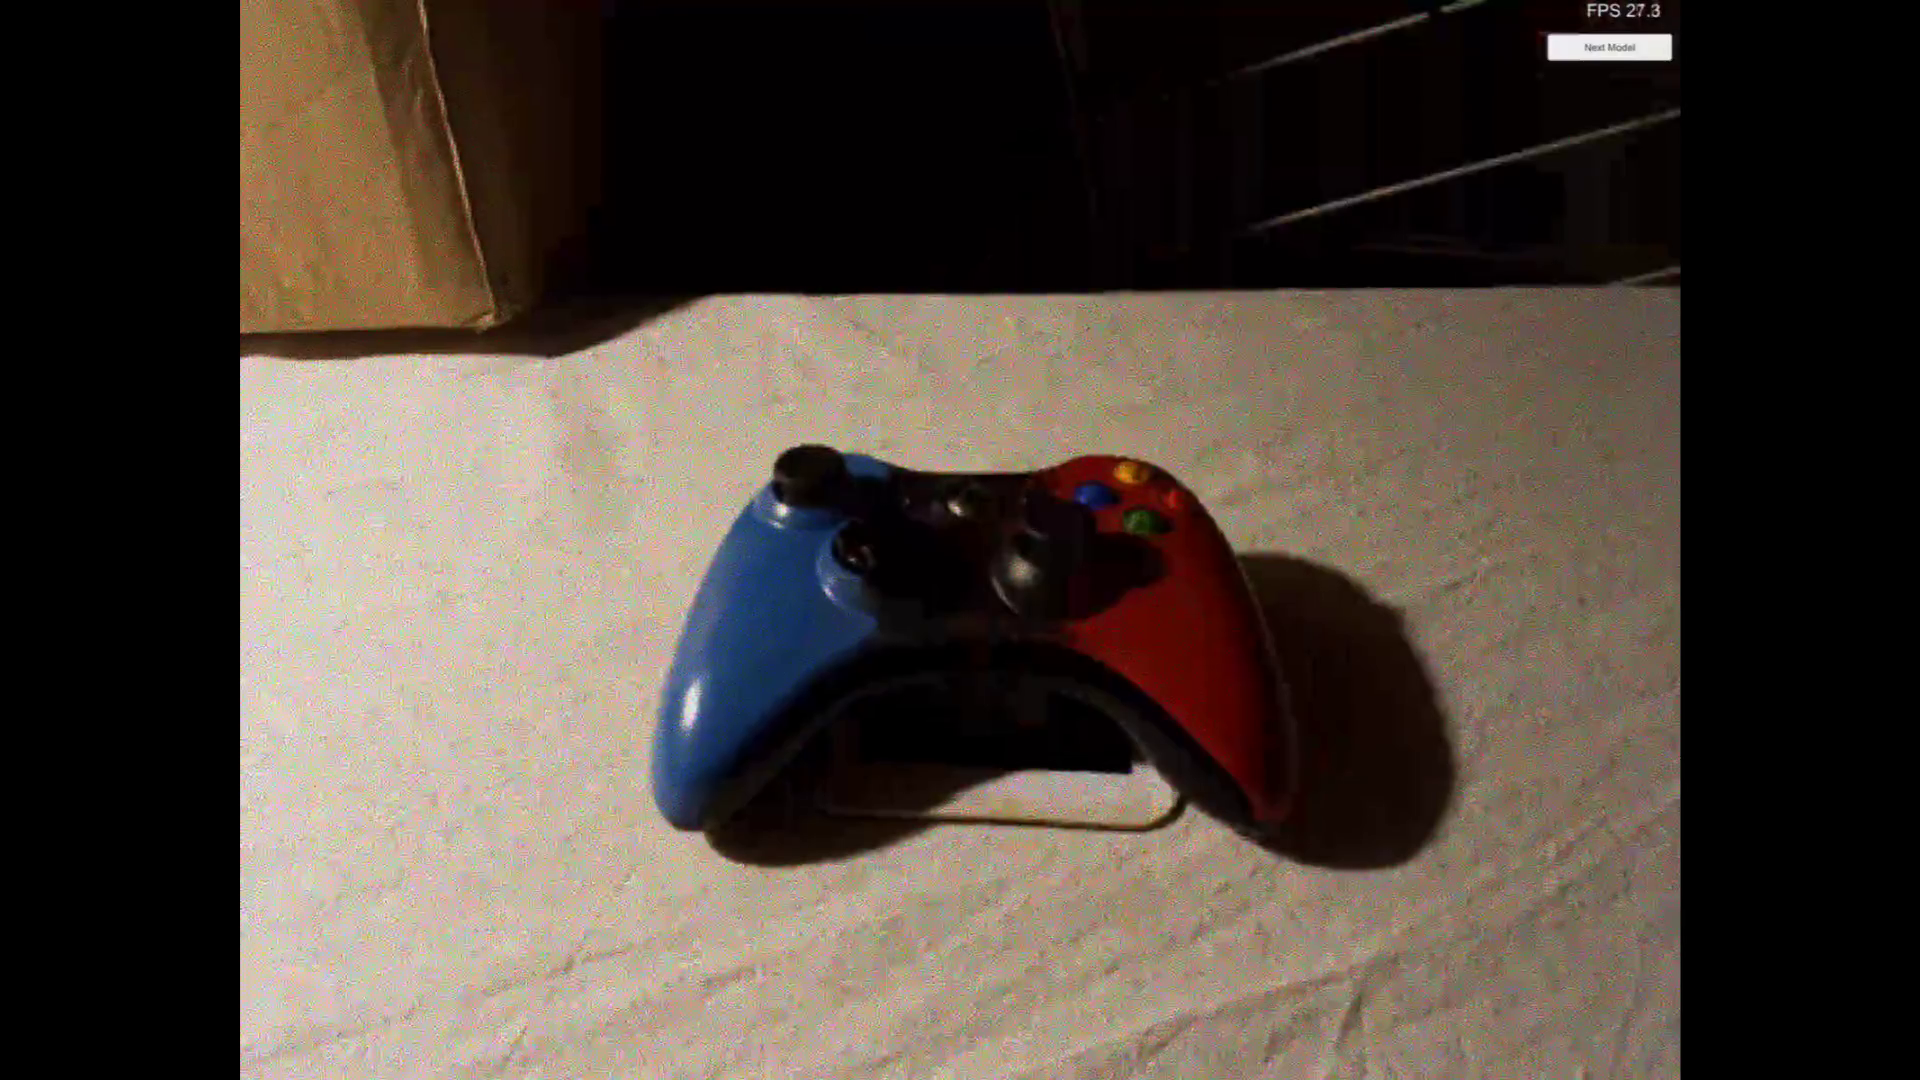
\includegraphics[width=0.99\textwidth]{Figures/ContReal.png} % first figure itself
        \caption{Real custom painted Xbox 360 controller}
    \end{minipage}\hfill
    \begin{minipage}{0.475\textwidth}
        \centering
        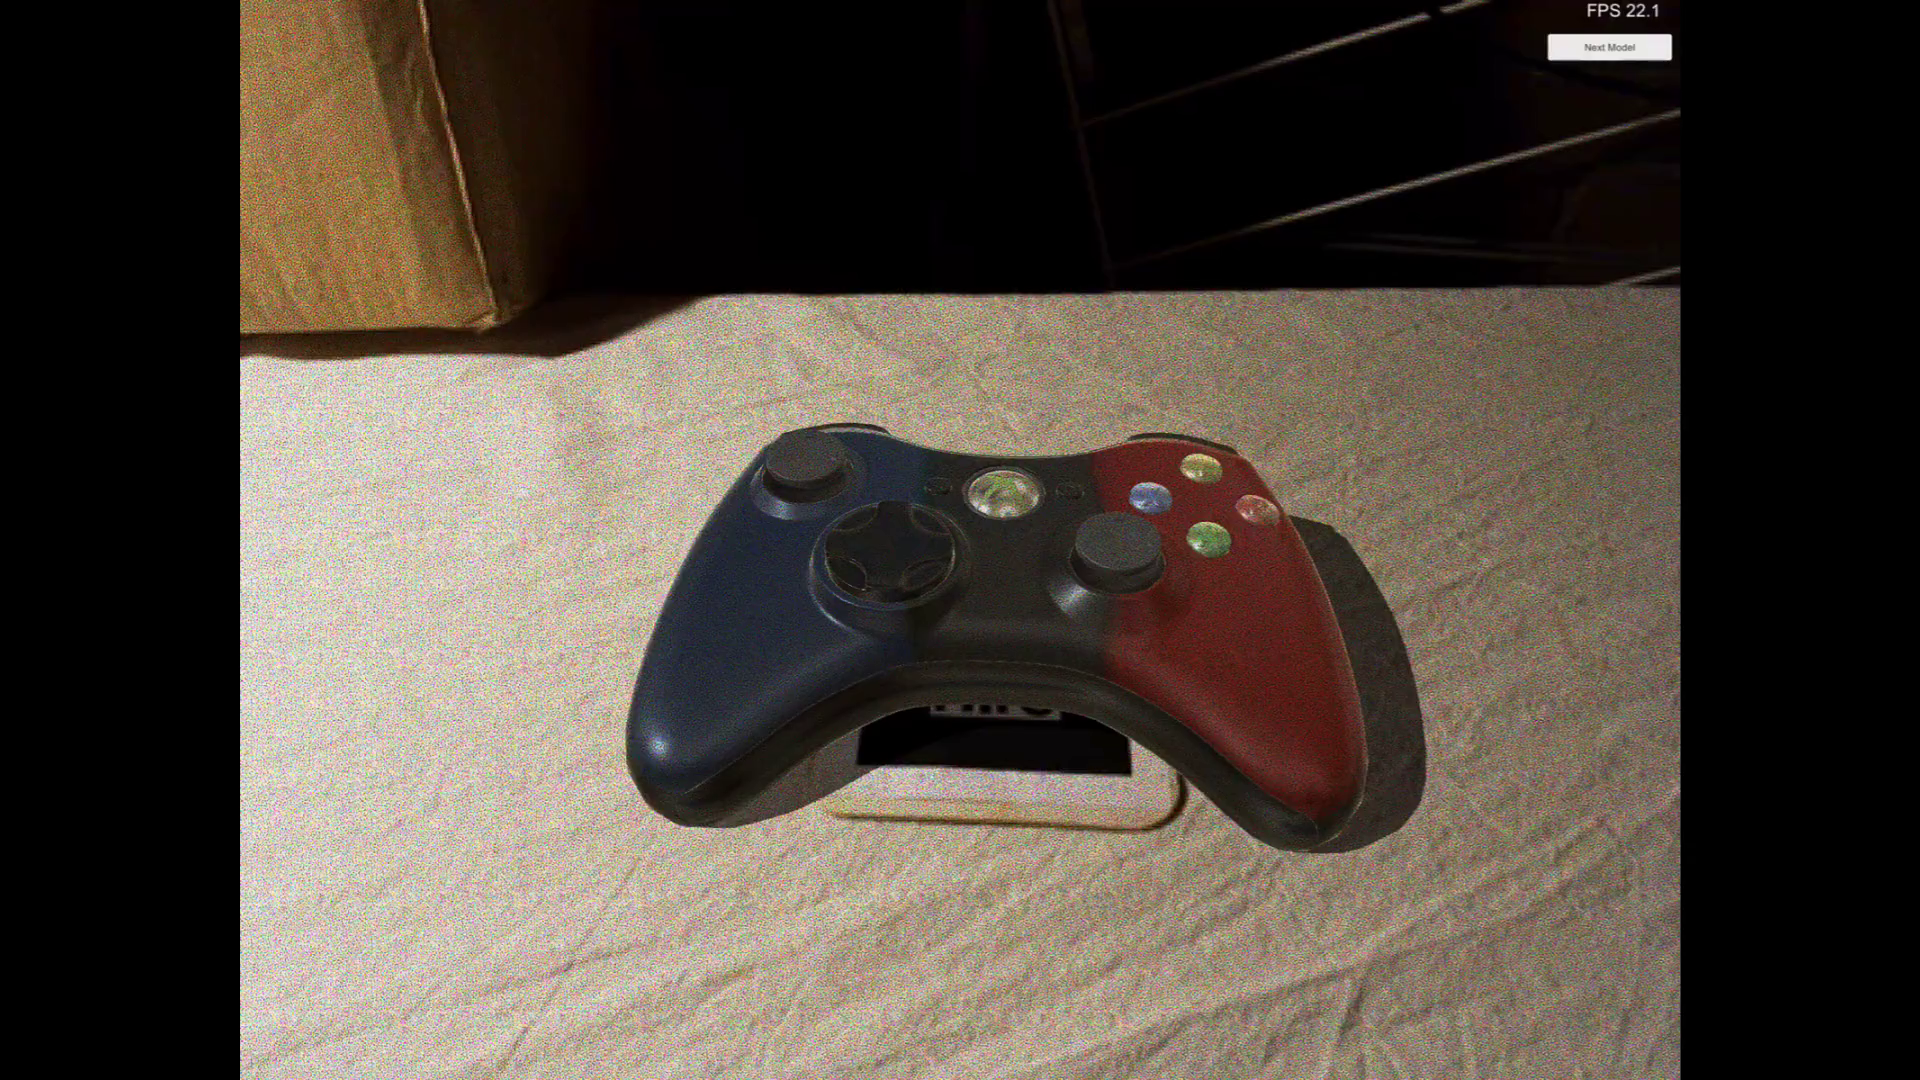
\includegraphics[width=0.99\textwidth]{Figures/ContVirtual.png} % second figure itself
        \caption{Virtual counterpart of the same object}
    \end{minipage}
\end{figure}

Experiment 2: Karsch's scenario  \newline
This scenario was hard to replicate, due to the unusual framing and placing of the objects. The image produced by this method is plenty different, and the method it's being compared with is not a runtime method, but even so there are conclusions that can be drawn. In the image produced by Karsch's application it's hard to say if the lighting in the real and virtual parts of the image really correspond, the light sources, except for one, are not present in the frame and there are no similar real objects to the virtual ones that would serve as ground truth. In this methods result there is enough evidence to prove that the lighting in both the real and virtual worlds is similar, with cues such as the presence of real objects and their shadow directions.\newline
In this methods application the framerate at 15 FPS is still quite acceptable considering that there are 6 virtual dense models, but given the fact that Karsch's method is not interactive there's no possibility to compare in this regard.
\begin{figure}[H]
    \centering
    \begin{minipage}{0.475\textwidth}
        \centering
        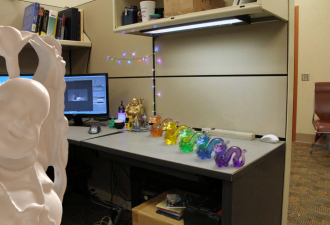
\includegraphics[width=0.99\textwidth]{Figures/budaDragonKarsch.png} % first figure itself
        \caption{Karsch's method results}
    \end{minipage}\hfill
    \begin{minipage}{0.475\textwidth}
        \centering
        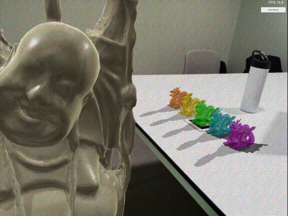
\includegraphics[width=0.99\textwidth]{Figures/budaDragon.png} % second figure itself
        \caption{This methods's results}
    \end{minipage}
\end{figure}


Experiment 3: Kanbara and Pessoa's scenarios\newline  
These two scenarios will be grouped together due to the fact that the steps to replicate the experiment are the same. They both presented ceramic material teapots with a lighting setting that they did not specify. 
\begin{figure}[H]
    \centering
    \begin{minipage}{0.475\textwidth}
        \centering
        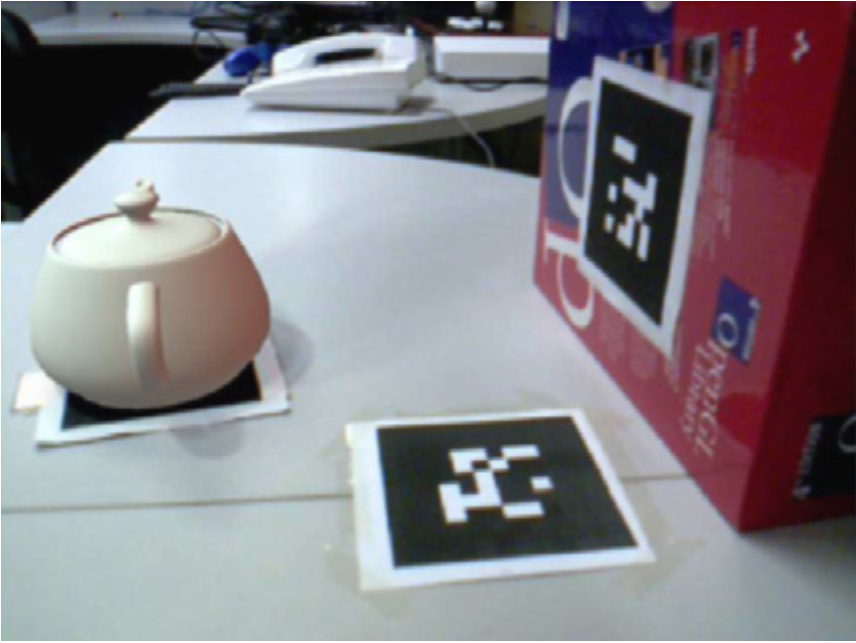
\includegraphics[width=0.99\textwidth]{Figures/Pessoa.png} % first figure itself
        \caption{Pessoa's method results}
    \end{minipage}\hfill
    \begin{minipage}{0.475\textwidth}
        \centering
        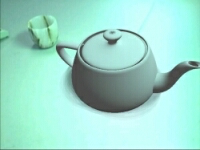
\includegraphics[width=0.99\textwidth]{Figures/kanbara.png} % first figure itself
        \caption{Kanbara's method results}
    \end{minipage}\hfill
\end{figure}

Both results look well blended into the environment, however in Pessoa's case it also must be said that the lighting setting is not disclosed and is not obvious from just looking at the results. For the aforementioned method there's also a considerable amount of pre-production required for the method to actually work, and the performance has a rather bad scaling, ranging from 180 FPS with no objects to 5 FPS with seven objects. The method in this work doesn't have those problems, the only pre-step required is to take a spherical panoramic image with the same device and no technical knowledge necessary;  and performance scales better going from 24 FPS with a single object to 15 with six of them.\newline
In the case of Kanbara's results they look really good, the downsides to their method that the one here resolves are the need for a physical 3D marker to probe lighting and the performance, they report 20 FPS on a computer for the experiment they published. It's admittedly a more than 10 year old computer at the time of this writing, but the method proposed here is achieving slightly better framerates on a mobile device.\newline

\begin{figure}[H]
    \centering
    \begin{minipage}{0.475\textwidth}
        \centering
        \includegraphics[width=0.99\textwidth]{Figures/pessoaComp.png} % first figure itself
        \caption{Pessoa's comparison results}
    \end{minipage}\hfill
    \begin{minipage}{0.475\textwidth}
        \centering
        \includegraphics[width=0.99\textwidth]{Figures/KanbaraComp.png} % first figure itself
        \caption{Kanbara's comparison results}
    \end{minipage}\hfill
\end{figure}

\section{Gallery}

Here are a few more screen captures from the application that show the potential of the method for the reader to draw their own conclusions.

\begin{figure}[H]
    \centering
    \begin{minipage}{0.475\textwidth}
        \centering
        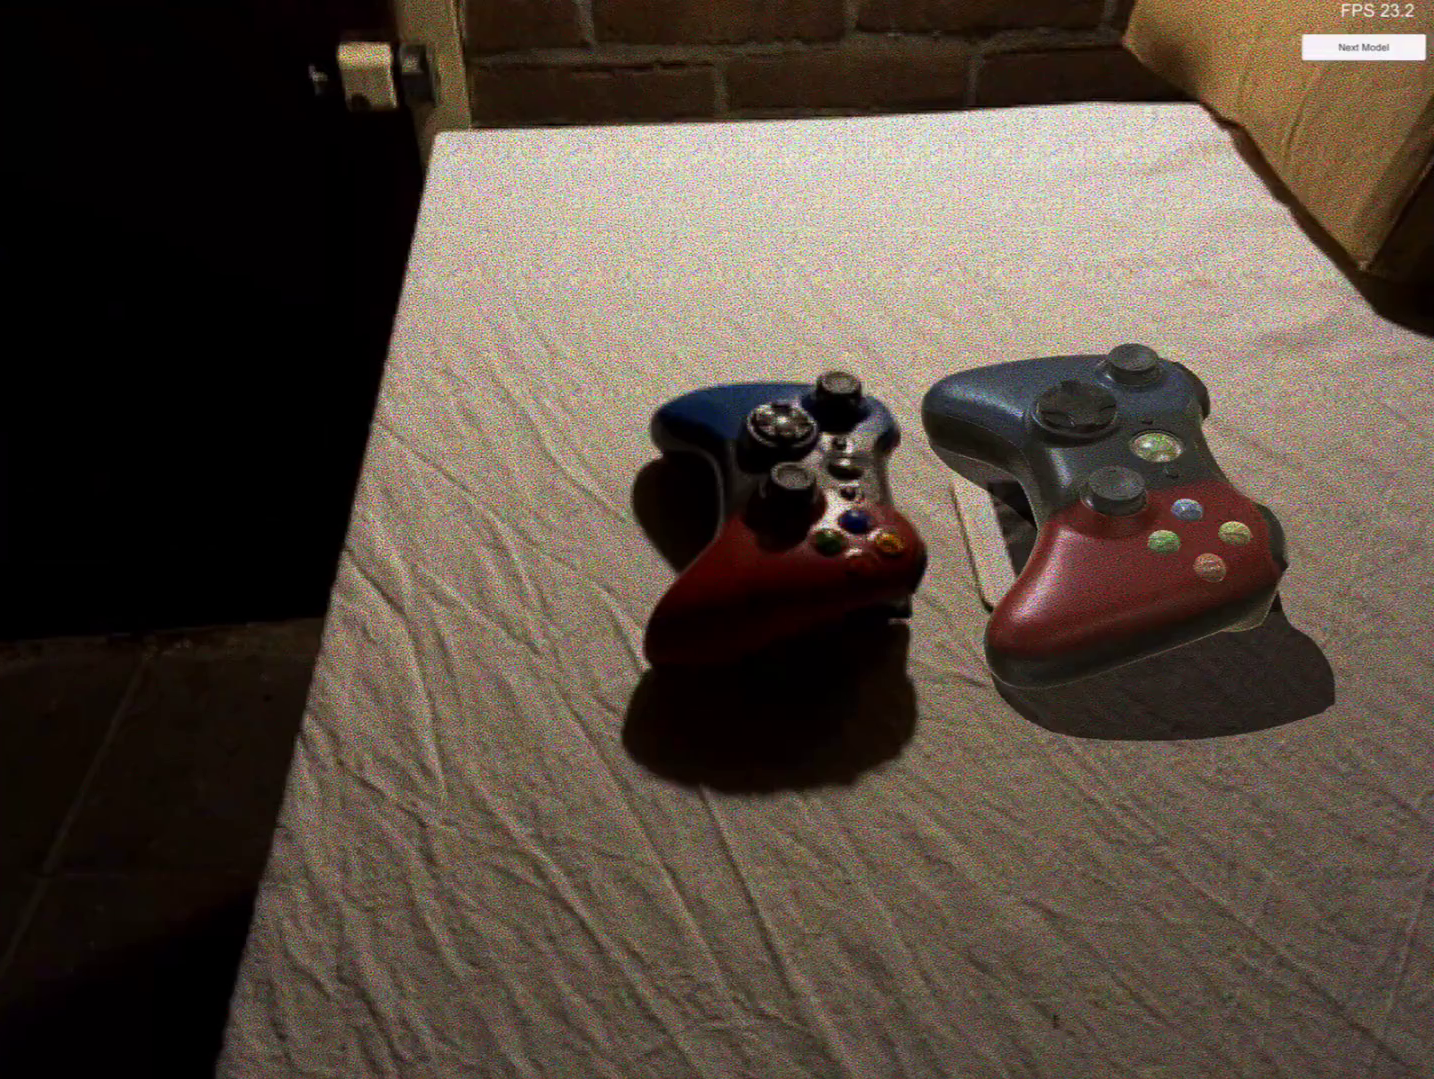
\includegraphics[width=0.99\textwidth]{Figures/ContBoth.png} % first figure itself
 
    \end{minipage}\hfill
    \begin{minipage}{0.475\textwidth}
        \centering
        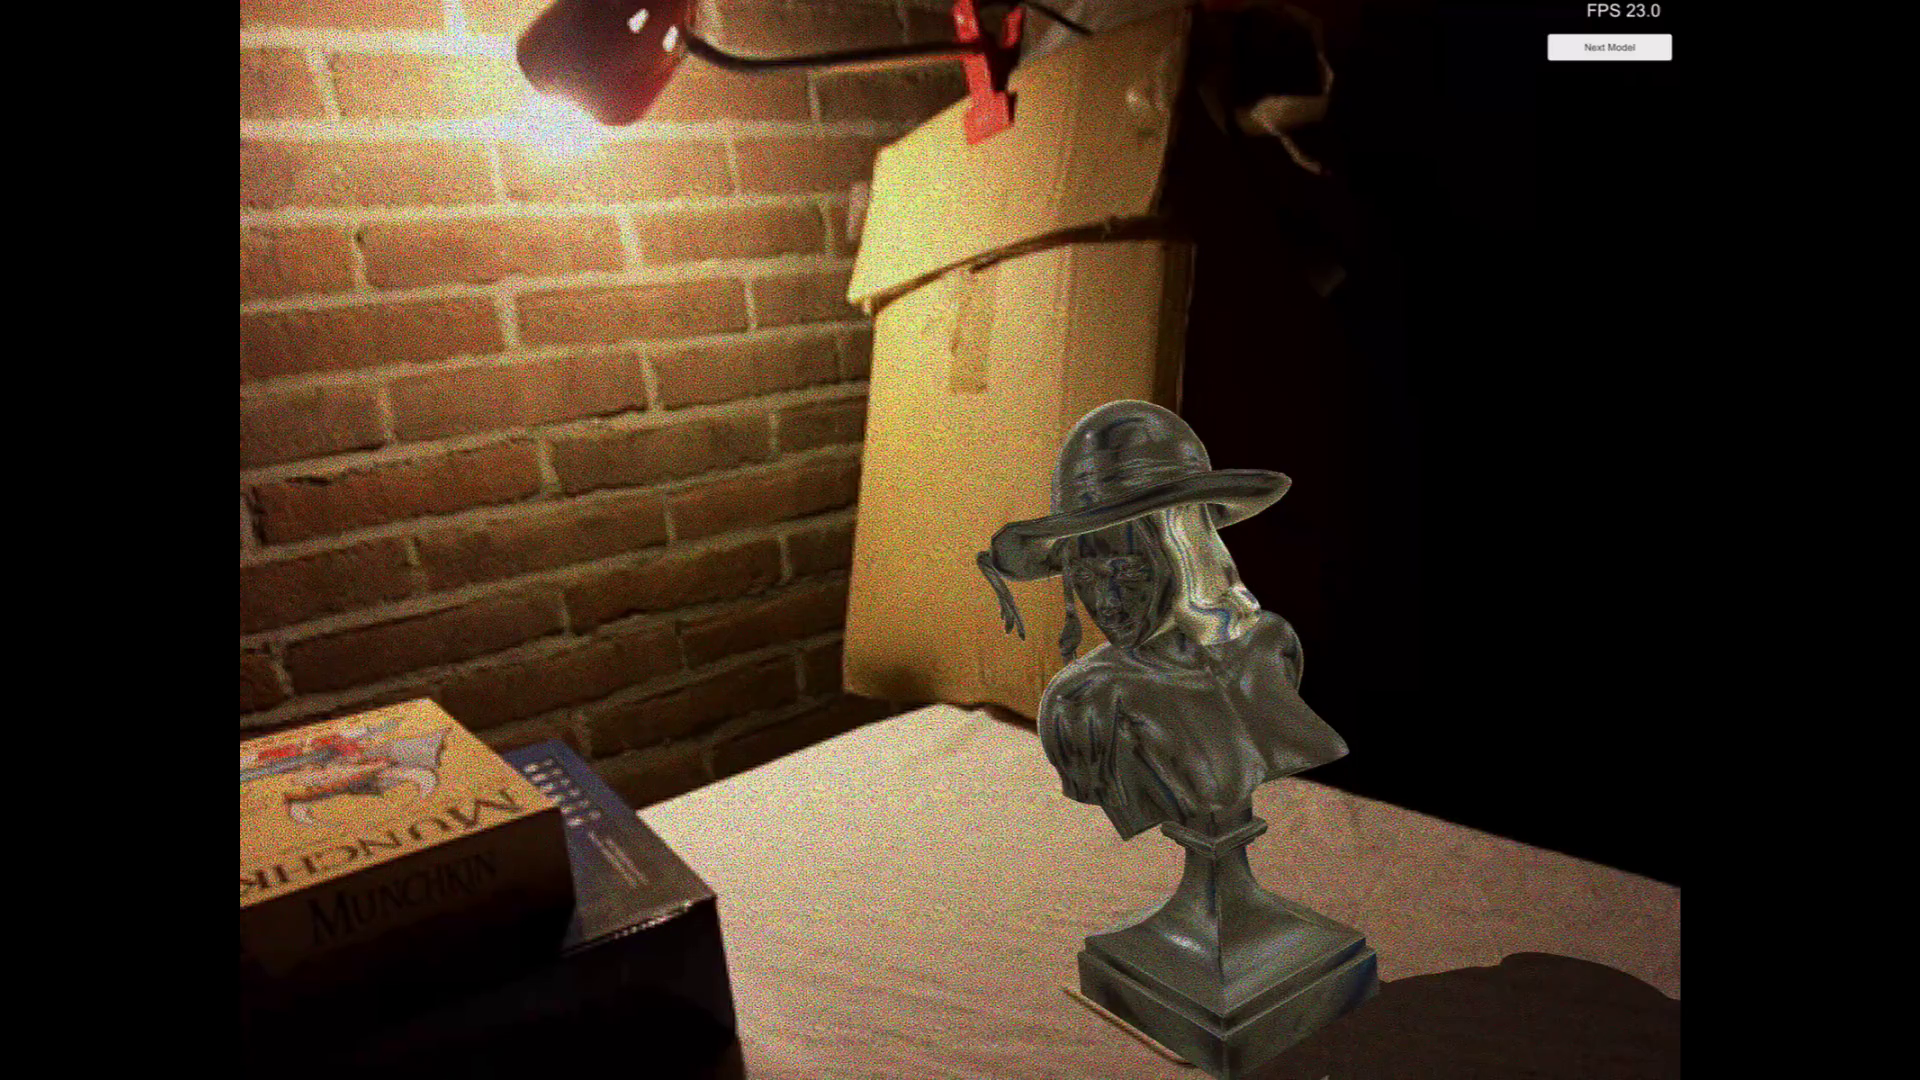
\includegraphics[width=0.99\textwidth]{Figures/Lena1.png} % second figure itself
    \end{minipage}\hfill
        \begin{minipage}{0.475\textwidth}
        \centering
        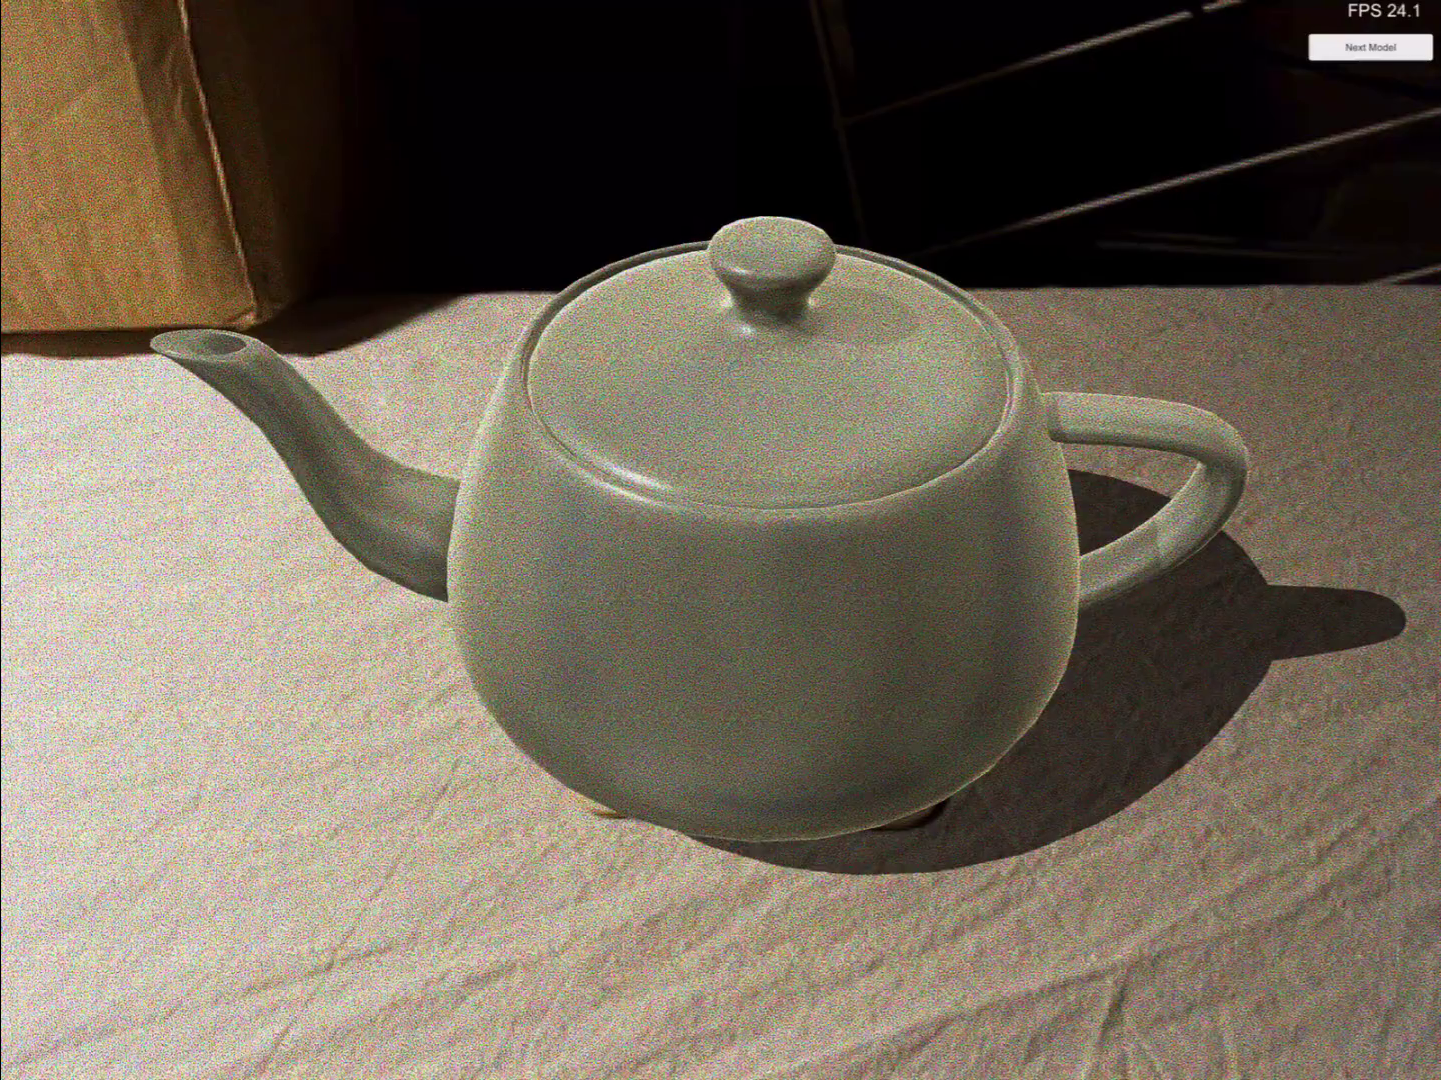
\includegraphics[width=0.99\textwidth]{Figures/TeapotVirtual.png} % second figure itself
    \end{minipage}\hfill
    \begin{minipage}{0.475\textwidth}
        \centering
        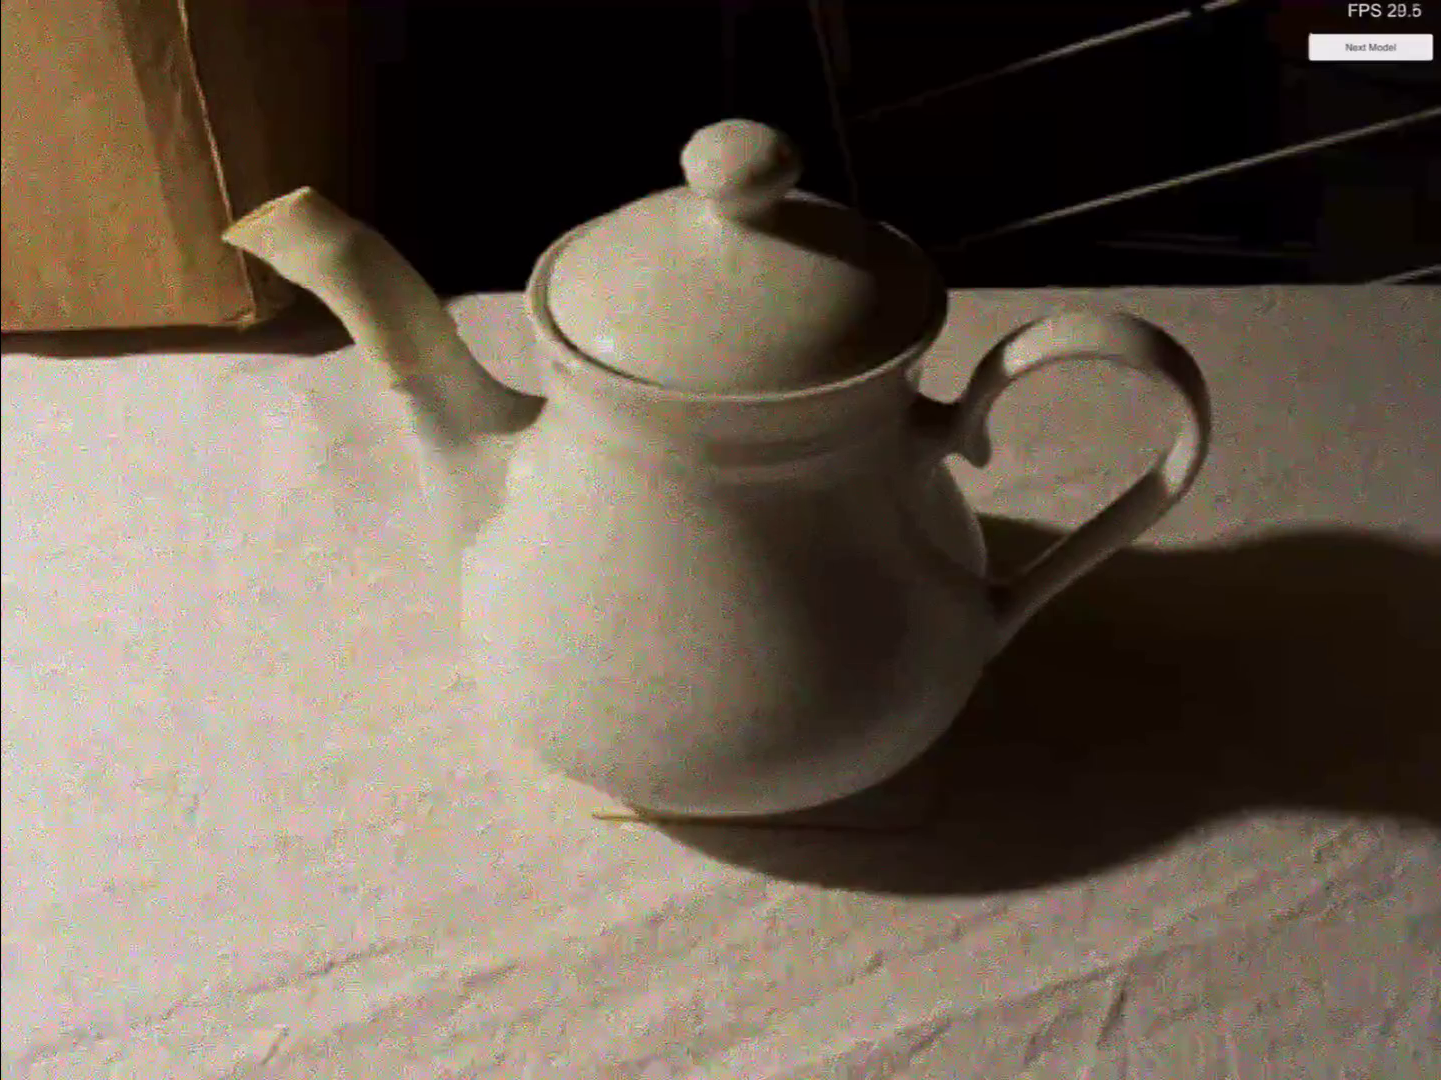
\includegraphics[width=0.99\textwidth]{Figures/TeapotReal.png} % first figure itself
    \end{minipage}
\end{figure}

\chapter{Discussion} \label{discussion}
In this chapter the results, discussed and a conclusion is formulated. The shortcomings of the method and the implementation are also mentioned and taken into consideration for future work.

\section{Discussion}
From the resulting images a very close resemblance among both virtual and real object can be appreciated, however it's still not a perfect fit. Some of the factors cannot be worked around trivially, for example one of the differences is that there are small imperfections present in the real object that are not there in the virtual one, in order to account for them, a 3D scan of the specific real object would be necessary. 3D scans are often extremely dense meshes that would pose a problem to maintain interactive framerates.\newline
Despite the film grain filter, it's still evident that the virtual camera has better resolution than the real one. The fact that in the virtual world everything looks "too perfect" also breaks the illusion of realism to a certain extent. However, in a real application of the method the user would ideally use AR to view something that is not there in the real world, instead of a side by side comparison to a real object. So by not having a clear ground truth of how such an object would look through the camera feed this problem is mitigated.\newline
Our method is placing lights using a reasonably accurate orientation, but at an admittedly inaccurate distance. After seeing the results we can also conclude that the orientation is far more important than the position, we do see differences in the length of the projected shadow, which is a determined by the distance to the light source, nevertheless this discrepancy is less noticeable than when the angle of the shadow is different from the real reference.

\section{Known shortcomings}
There are a few known cases where false positives are found by the light detection algorithm. When a light source is directed towards a glossy surface, such as a varnished desk for example, the incidence of the light on such a surface is detected as a light source as well. A similar thing happens sometimes for intense white objects that are not light sources. Although in the first scenario it can be argued that the light bouncing off a glossy surface could indeed be considered a light source. The system is closed once the runtime phase starts, therefore it lacks adaptation to light changes, due to the nature of the method, having a pre-calculation phase and a runtime phase, it wouldn't be possible to change the light setup in the same way as it was originally captured.\newline
The system limits the amount of lights it simulates to 8 for performance reasons, but even at 8 light sources the performance of the application is low. Between 15 and 24 FPS, it can still be considered interactive, but it's not ideal, specially when taking into account that the application is only doing rendering, a real application of the method, such as a game, would require other layers of complexity that would need processing time.\newline
When virtual shadows overlap a real object that is in front of it the result is not visually pleasing or realistic. In order to prevent this and make the shadow cast on non-planar neighboring objects, or at least have the objects occlude it, some knowledge of the environment in 3D would be necessary, and most likely that would require hardware that is not present on average consumer smartphones.

\section{Conclusion}
All in all, despite the shortcomings of the method the objective was achieved. The main goals of the method are to approximate the lighting conditions of the environment via a panormaic image and to use this knowledge of the environment to improve the realisim of the rendering. Both objectives are met, in the understanding that improvement is not an absolute measure, meaning that as long as the method makes the composted scene more realistic the objective is fulfilled, regardless of being far from perfection still.\newline
There's room for improvement, both on the technical side, on the user experience side and in the results. This will be further developed in the next section.

\section{Future work}
During the development of this method there were several changes to the Augmented Reality landscape through the introduction of new SDK's by Apple and Google. ARKit by Apple and Tango/ARCore by Google are much more robust solutions than the ARToolKit used in this method. While both ARKit and ARCore have an ambient light estimation feature, and ARCore supposedly even has direct illumination estimation, the overlap with what was proposed here is not complete. In a future iteration of the system it would be interesting to see the method working with these new SDK's. Google Tango would be even more interesting, due to the fact that it has a depth sensing camera, so it would even be possible to roughly reconstruct the scene for accurate shadow casting and determine the distance to light sources precisely.\newline
Other than that, a vast improvement would be support for changing light conditions. Most real-world applications for such AR graphics would require interaction outdoors for more than a few minutes, so the lighting conditions are bound to change in the middle of a session.\newline
Just for the sake of maintaining a more uniform user experience it would be a nice addition to implement something similar to the Google Street View spherical panorama capture module within the app. This is something completely off-topic for the method and something not trivial to implement, but if it was there it would be a nice addition nonetheless. 

\clearpage

\bibliographystyle{apalike}
\nocite{*}
\bibliography{references}
\end{document}
